\section{Risultati dello swing-up}
% LQRegulatorGains[
% ssm /. params, {Q, R} /. {r11 -> .05, q11 -> 2} /. params]
% THIS is kinda what I used for the swing up.

\subsection{Simulazioni e parametri}
La strategia di controllo~\eqref{eq:control-strategy-tanh} non
mi garantisce di riuscire ad eseguire lo swing-up rimanendo nei
limiti fisici del sistema (la lunghezza della rotaia).
Considerando i parametri del motore, fisso un limite conservativo
\todo{ref i parametri del ,motore}
per la forza massima che questo può esercitare:
\begin{equation*}
    f_{\max} = 5N.
\end{equation*}
Approssimo l'accelerazione del carrello come
\begin{equation*}
    a \approx \frac f {M + m}
\end{equation*}
e trovo una stima per $a_{\max}$:
\begin{equation*}
    a_{\max} \approx \frac {f_{\max}}{m+M} \approx 20 \frac m {s^2}.
\end{equation*}
La simulazione in \autoref{fig:swingup-overflow} mostra che,
con questa scelta di parametri, il sistema
reale non raggiungerebbe
l'intervallo di controllabilità prima della fine della rotaia.

\begin{figure}[h]
    \centering
    \begin{subfigure}[]{\textwidth}
        \centering
        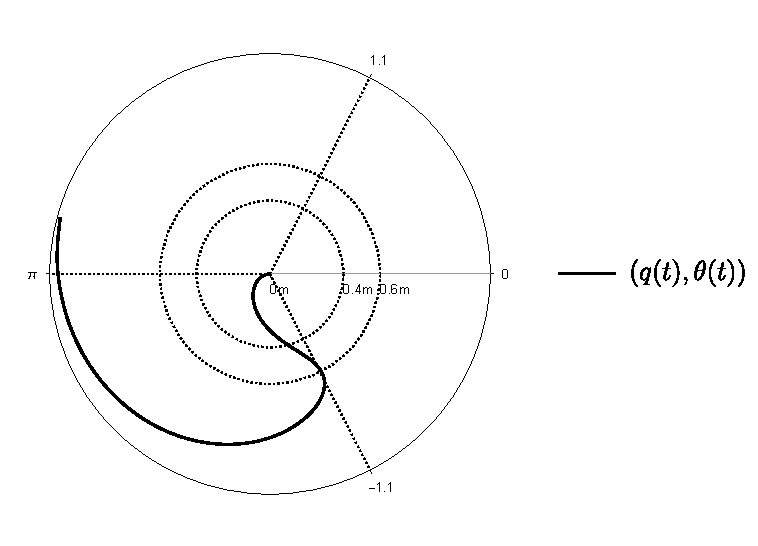
\includegraphics[width=.8\textwidth]{assets/polar-swingup-simulation}
    \end{subfigure}

    \caption[sssss]{
        ssssss
    }
    \label{fig:swingup-overflow}
\end{figure}

Ho risolto questo problema adottando alcuni accorgimenti.
\begin{itemize}
    \item A parità di accelerazione, il motore trasferisce più
    energia al pendolo quando $|\theta| \approx \pi$\footnotemark.
    Ho quindi fissato un intervallo per $|\theta| < \theta_{\min} $ in cui il
    controllo è azzerato.

    \item Al posto di controllare il sistema verso $E = 0$,
    controllo il sistema verso un energia positiva $E \to \Delta E$.
    In questo modo ho un piccolo margine per tenere conto di attriti
    e altri fattori non modellati.

    \item Ho usato una strategia di stabilizzazione più aggressiva,
    così da ridurre lo spazio che il carrello deve percorrere prima
    di tornare verso $q = 0$.
\end{itemize}

\footnotetext{Per convincersene, è sufficiente studiare l'andamento
della~\eqref{eq:dvdt} per un valore abritrario di $\dot \theta \neq 0$.}
I parametri finali che ho usato per il sistema reale sono riportati
in \autoref{tab:parametri-swingup}

\todo{TABELLONA PARAMEtri SWUP}


\subsection{Comportamento del sistema}
Il sistema reale riesce ad eseguire lo swing-up.
In base alle condizioni esterne\footnotemark, si osservano due
comportamenti possibili:
\begin{enumerate}
    \item il pendolo viene portato in posizione verticale in un
    singolo movimento, oppure
    \item il pendolo viene fatto oscillare prima di raggiungere la
    posizione verticale.
\end{enumerate}
L'osservazione di uno dei due comportamenti dipende
dalla forza massima che il motore riesce ad esercitare sul carrello.
Se la forza è abbastanza alta, si osserva il comportamento~(1),
altrimenti il comportamento~(2).

Riporto in \autoref{fig:swingup-real-one} solamente i dati relativi al comportamento~(1), in quanto sono
sufficienti per mostrare la logica seguita dall'equazione~\eqref{eq:control-strategy-tanh}.
Una descrizione più dettagliata di tutti i possibili casi è disponibile in
%todo cite paper swingup

\footnotetext{La temperatura esterna influisce leggermente
sia sui parametri del motore, sia sugli attriti dei cuscinetti,
    cambiando i parametri del sistema.}

\begin{figure}
    \centering
    \begin{subfigure}[]{\textwidth}
        \centering
        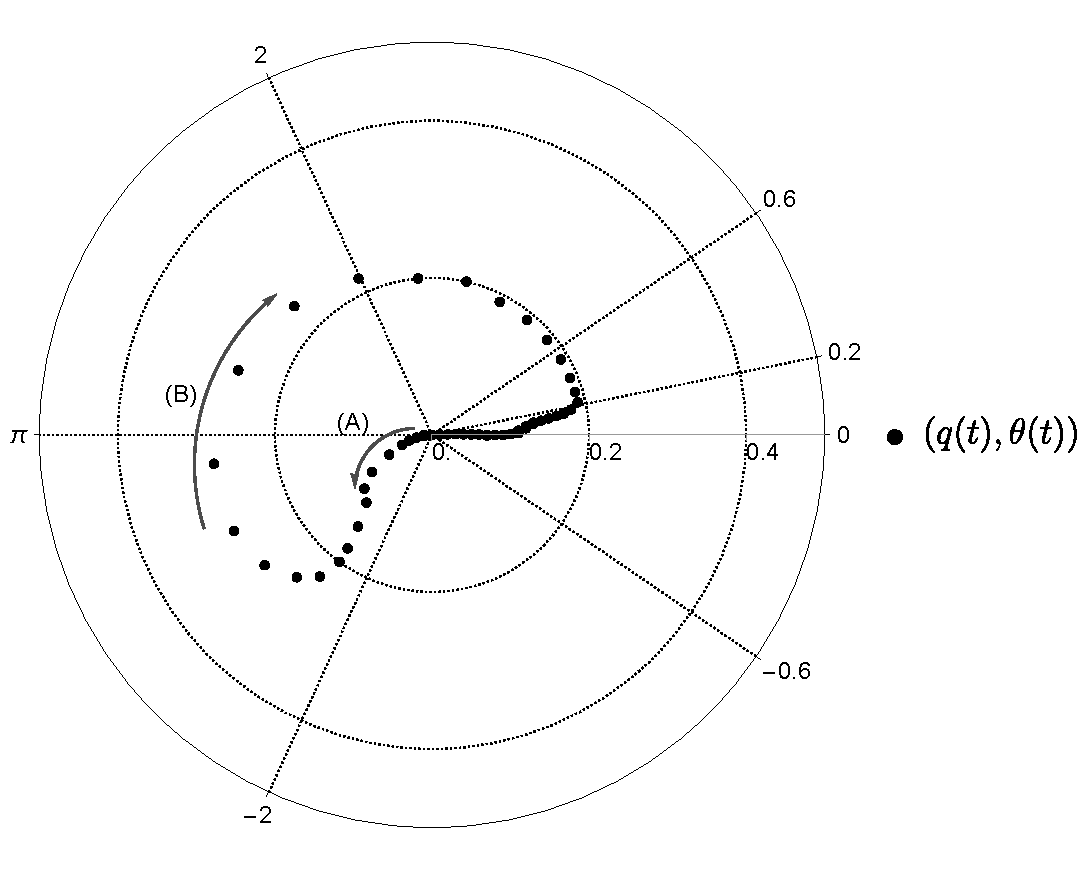
\includegraphics[width=.75\textwidth]{assets/polar-swingup-real}
        \caption{Posizione del carrello e angolo del pendolo.
        La posizione è riportata sull'asse radiale. In questo
        caso particolare, il moto è
        completamente contenuto nella regione $q > 0$
        }
    \end{subfigure}
    \\[5ex]
    \begin{subfigure}[]{\textwidth}
        \centering
        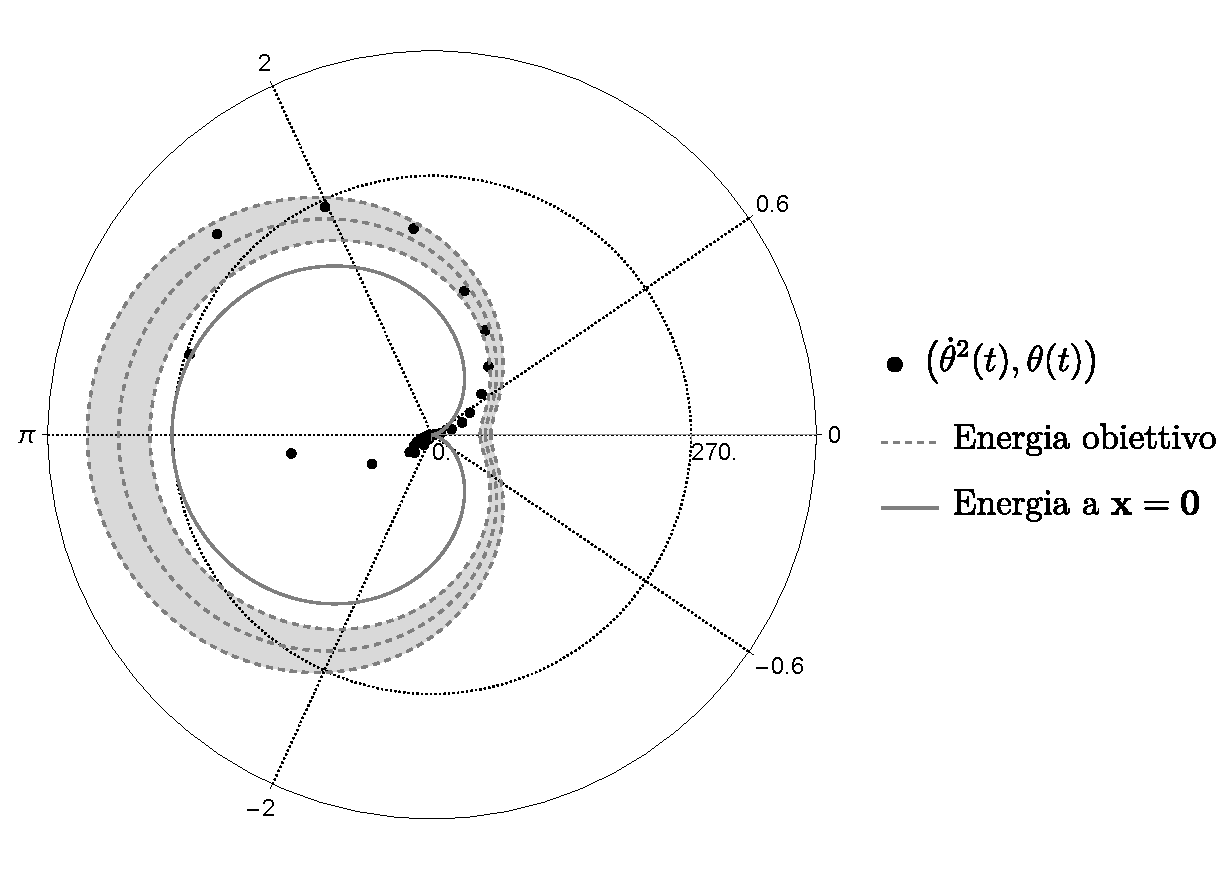
\includegraphics[width=.8\textwidth]{assets/polar-swingup-energy}
        \caption{Energia del pendolo in funzione di angolo e
        velocità angolare quadratica.
        La velocità angolare elevata al quadrato è riportata sull'asse
        radiale.
        }
    \end{subfigure}

    \caption[SSSS]{
        SSSS
    }
    \label{fig:swingup-real-one}
\end{figure}


\todo{add proper figure description}

